\chapter{静态分析混淆技术研究与实现}
%第四章内容
逆向攻击者在分析软件时通常会通过动态分析工具如OllyDbg、WinDbg、SoftICE等工具和静态分析工具如IDA工具来分析软件,动态分析工具是在运行是分析可执行程序,可以观察到程序执行时的寄存器、堆栈、内存空间等的所有数据。静态分析工具则是直接反汇编源码,它的优点是对代码阅读者提供更多的信息,高级功能的静态分析工具比如IDA甚至可以直接由汇编代码得到与源码类似的C语言代码,函数的所有跳转都给出详细信息。

本节将针对静态分析工具对软件进行反调试保护,提出一种建立索引进行函数间基本块交换的混淆算法,最后根据提出的算法实现了一个PE文件保护器。
\section{常用的反调试技术}
\label{cha2:sec:techarch}

常见的反调试技术有使用花指令、文件完整性检验、代码与数据结合、调试器检测等。

逆向工程是研究程序以获得有关其工作方式和使用的算法的封闭信息的过程,尽管软件逆向可用于合法的研究目的,尤其是恶意软件分析或未记录的系统研究,但通常认为是黑客将其用于非法活动,调试与反调试一直都是软件保护者和软件破解者之间的相互博弈,虽然理论上不存在不能被逆向分析破解的程序,但是软件保护者们依然采用各种各样的方式来实现对软件的保护,逆向工程的工作中也没有最优解。本课题也只是在加大破解难度的原则上对软件进行保护,并加入自己的加密算法,最终加大破解难度或者引导破解者到错误的方向。本节将简述常见的的基本保护措施,并会加以改进。

常见的分析软件的方法有:一、使用数据包嗅探器进行数据交换分析,以分析通过网络交换的数据。二、软件二进制代码反汇编以汇编语言形式列出其代码。三、反编译二进制或字节代码,以高级编程语言重新创建源代码。本课题考虑了流行的反破解和反逆向工程保护技术,即Windows中的反调试方法。我们一开始就应该提到,不可能完全保护软件免受逆向工程。各种反逆向工程技术的主要目标只是使过程尽可能复杂。

\subsection{花指令}

花指令是一种隐藏不需要进行反向工程的代码块或其他功能的方法。在实际代码中插入一些垃圾代码还可以确保原始程序的正确执行,并且程序无法很好地进行反编译,难以理解程序的内容并难以达到使代码混乱的效果,使用某种方式排布数据和代码,在汇编代码中插入一些“数据垃圾”,对反汇编软件进行干扰。

第一种花指令利用了汇编指令的长度。不同的体系结构的机器指令长度并不相同,有多操作码指令和单操作码指令的区分,多操作码指令需要确定这条指令第一个字节的起始位置,由于长度固定,所以指令的结尾也是固定的,否则可能会被反编译器翻译为其他的或者错误的指令。图\ref{huazhilinga}是一段汇编代码。

\begin{figure}[htbp]
	\centering
	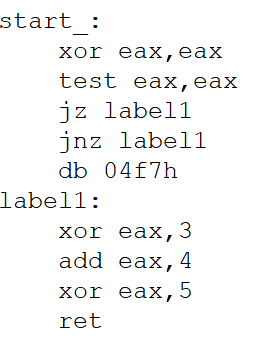
\includegraphics[width=4cm]{huazhiling.png}
	\bicaption{花指令汇编源码}{Flower instruction assembly source code}
	\label{huazhilinga}
\end{figure}


对源程序使用nasm编译,使用W32Dasm反汇编,结果图\ref{huazhliingb}。

\begin{figure}[htbp]
	\centering
	\centering
	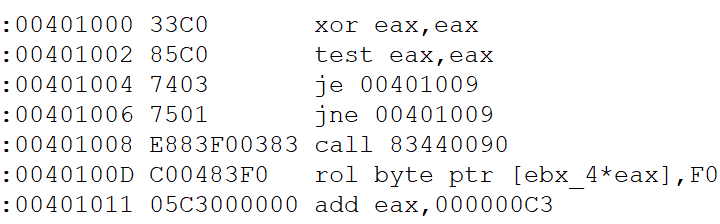
\includegraphics[width=10cm]{huazhilingb.png}
	\bicaption{反汇编硬编码代码}{Disassemble hardcoded code}
	\label{huazhliingb}
\end{figure}

W32Dasm使用的反汇编器是逐行反汇编的,代码中的04F7h不是任何汇编指令,干扰了W32Dasm使用的Linear Sweep反汇编引擎,对指令的起始位置做出了错误的判断,使反汇编的跳转指令的跳转位置无效。比如00401009h这个位置属于指令的内部,不具有反花指令引擎的反汇编器很容易给调试者带来无效的分析信息。

反汇编引擎最关键的问题之一是代码与数据的区分,由于汇编代码的指令长度是不同的,并且代码之间存在绝对地址和相对地址,跳转命令可能使用这些地址来直接跳转或间接跳转,所有反汇编引擎要对所有指令的长度和功能有确切的认知,从而保证反汇编结果正确性。

第二种花指令是利用了将JMP指令修改为JE+JNE(JX+JNX或者JZ+JNZ等)实现的。

在汇编语言中存在着大量的条件跳转,比如JNE是比较两个操作数,如果不相同,则跳转,如果不同,则不跳转,JE与上述指令功能相反。条件跳转都是成对出现的,比如JZ/JNZ、JX/JNX等。而JMP指令则是无条件跳转,使用方法为JMP XXXX,指令运行时永远会跳转到XXXX处,JMP这条指令的地址和XXXX代表的地址中间的代码可能永远不会被执行,这部分代码叫做DEAD CODE。JE+JNE型代码与JMP代码同理,如果将JE和JNE代码同时使用,将会实现无条件跳转。

\begin{figure}[htbp]
	\centering
	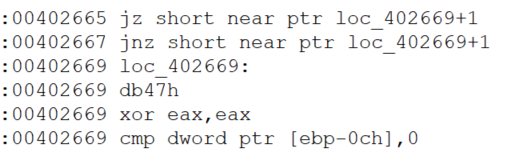
\includegraphics[width=9cm]{jnz.png}
	\bicaption{跳转花指令}{Jump flower instruction}
	\label{jnz}
\end{figure}


如图\ref{jnz}所示,无论标志位是否为1,代码都会跳转到00402669处执行,代码都会跳转到00402669处执行 47h指令,也就是无用代码。db 47h指令则会给反编译器带来困扰,因为这行代码是在代码区域,但是不能被识别为指令。

第三种花指令的抗逆向效果较低,但是这部分指令不会影响其他部分有用程序,对程序的影响较小,植入的成本更低,程序不容易出现错误。这种花指令通常构造一部分没有意义的算术运算。

%第一行和第二行都是EBX加2,第五行EBX加上1,第七行EBX减1,所以EBX的值并没有发生变化;第三行的NOP,无意义代码;第四行EAX加28,第六行EAX加上负28,所以EAX的值也没有被改变。这种垃圾指令是最常见的花指令,通常可以使用脚本自动去除这种花指令,干扰的效果较低,但是如果添加大量的这种指令仍然可以给逆向分析者带来麻烦。

\subsection{文件完整性检验}

在抗逆向方案中,文件完整性检验是最基础的方案,通常也被最先考虑并采用。文件完整性检验就是在软件运行过程中,对本文件进行自身完整性的检查,抵御逆向分析者对文件进行修改,可以达到一定的抗分析目的。

文件完整性检验原理就是在发布时预先计算文件的哈希值,存放在程序的启动代码中,在文件每次运行时,首先对当前文件的某个模块或者全部模块进行哈希运算得出哈希值,与预先计算好的哈希值对比,如果相同则成功执行,如果不同则直接终止程序。

文件完整性检验通常使用三种方式,分别是:磁盘文件校验的实现、内存映像校验和校验和。

其中的校验和方式安全性能较差,在PE文件的IMAGE\_OPTIONAL\_HEADER中有一个校验和(Checksum)字段,这个数据结构中已经存放着整个文件的校验和,相当于PE文件对自身的一种保护,但由于这种保护广为人知,现在几乎已经失去它的作用,只要逆向分析者发现有校验和的检查,自己手动修复校验和或者使用工具修复都可以成功绕开这个限制。
%Windows提供了一个API函数来检测校验和,其原型如下图

%图657

%\subsection{常量分解}

%常量分解就是对一些寄存器中存储的常数值进行展开,对常数进行分解,可以使程序的运行更加复杂,在下图 中 两条指令分别是将3赋值给EBX和将4096赋值给EDX。4096字节为4K,大小为一个页。如图a中4096可以得出这段代码很可能是4K大小的一个数组。图b为图a的展开后的结果,第一行指令将1000赋值给EBX,第二行加16后EBX等于1016,第三行将EBX逻辑右移9位,1016向逻辑右移动9位后刚好位1;第四行将1赋值给EDX,然后将第五行将EDX逻辑左移12位,正好是4096大小。

%图

%常量展开就是将常量以一种复杂的方式再计算一遍,最后的结果相同,虽然这样会加大程序的运行时间,并且实现的复杂度比较高,不利于代码的优化,但也一定程度上影响逆向分析者的工作量。


\subsection{调试器检测}

\subsubsection{使用IsDebuggerPresent}

提出的反调试方法是基于IsDebuggerPresent函数。此函数检测调用模式是否正在由用户模式调试器调试。图\ref{isdebug}的代码显示了基本保护的示例:

\begin{figure}[htbp]
	\centering
	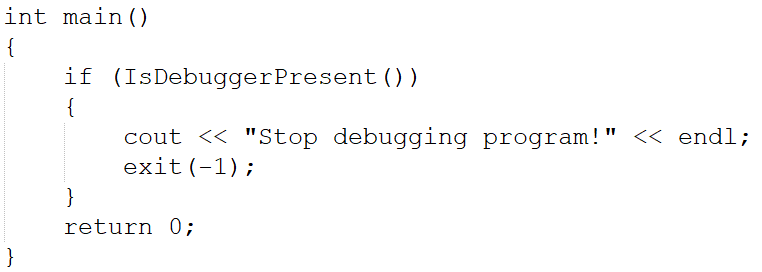
\includegraphics[width=10cm]{isdebug.png}
	\bicaption{IsDebuggerPresent函数}{IsDebuggerPresent function}
	\label{isdebug}
\end{figure}

%如果看一下IsDebuggerPresent函数内部,将会发现一下代码:

%\begin{lstlisting}
	
%	0:000< u kernelbase!IsDebuggerPresent L3
%	KERNELBASE!IsDebuggerPresent:
%	751ca8d0 64a130000000    mov     eax,dword ptr fs:[00000030h]
%	751ca8d6 0fb64002        movzx   eax,byte ptr [eax+2]
%	751ca8da c3              ret
%\end{lstlisting}

%对于X64进程

%\begin{lstlisting}
%	0:000< u kernelbase!IsDebuggerPresent L3
%	KERNELBASE!IsDebuggerPresent:
%	00007ffc`ab6c1aa0 65488b042560000000 mov   rax,qword ptr gs:[60h]
%	00007ffc`ab6c1aa9 0fb64002           movzx eax,byte ptr [rax+2]
%	00007ffc`ab6c1aad c3                 ret
%\end{lstlisting}

%PEB(过程环境块)结构相对于fs段偏移了30h(对于x64系统,相对于gs段偏移了60h)。如果我们查看PEB中的2偏移量,则会发现该BeingDebugged字段:

%\begin{lstlisting}
	
%	0:000< dt _PEB
%	ntdll!_PEB
%	+0x000 InheritedAddressSpace : UChar
%	+0x001 ReadImageFileExecOptions : UChar
%	+0x002 BeingDebugged    : UChar 
%\end{lstlisting}

\section{建立索引进行函数间基本块交换的混淆算法}

本节将会提出一种对混淆算法,此算法对二进制函数分块,进行交换,并建立函数块之间交换记录的索引。目前市面上大部分混淆算法都是对一个函数的二进制进行加密处理,比如对函数内部的汇编代码进行花指令处理或进行分块然后进行交换。由于函数内部的二进制代码可能极其复杂,函数之间进行块交换的主要困难在这几个方面:一、编程难度大,由于只能看到函数的二进制代码;二、虽然通过反汇编处理后可以看到汇编代码,但是在编程时需要分析各条指令的长度、函数执行时的栈帧结构的保护、执行时内存堆空间的变化情况。

本节将会提出相对简单的二进制混淆方式,只考虑移动函数内部二进制命令中较易处理的汇编命令,比如MOV、SUB、ADD等不影响栈和堆的汇编指令,且这些指令的长度大部分是固定的,后文将会实现这种算法,并进行分析。

\subsection{基本思想} 

一个可执行程序中包含多个函数,函数之间可能进行相互调用,首先要对函数进行分块处理,把每个函数切分为可交换块和不可交换块,可交换块数量大于等于一,在移动时只会移动可交换块,故不考虑不可交换块块数。通常,函数的指令都是连续的,函数的调用流程反映了程序的执行时的运行结构。

在记录交换索引的基础上,对函数之间的可交换块进行了的交换,在可执行文件的尾部建立一个新节来存储索引信息。

\begin{figure}[htbp]
	\centering
	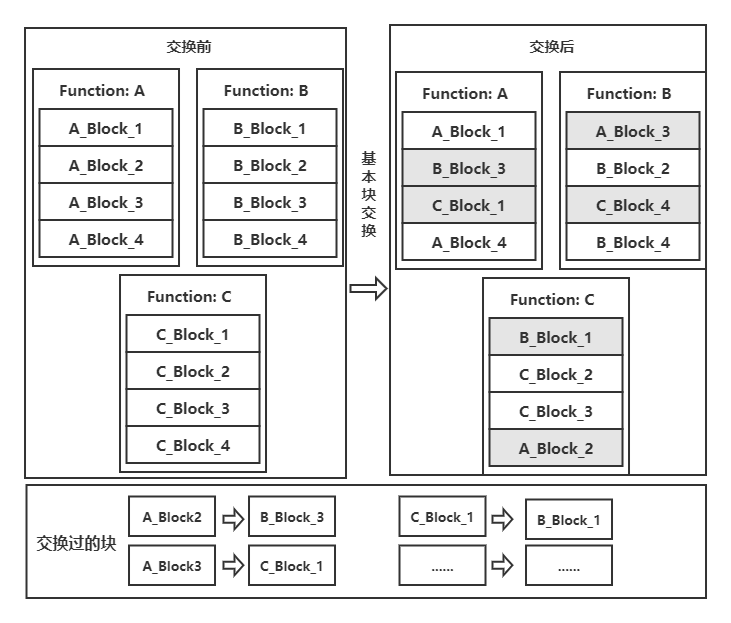
\includegraphics[width=13cm]{switch.png}
	\bicaption{建立索引进行函数间基本块交换过程}{Establish an index for the basic block exchange process between functions}
	\label{switch}
\end{figure}

如图\ref{switch}所示,图中展示了三个函数块的交换过程,并在左侧建立索引,在恢复时程序会根据此索引进行函数执行流程恢复。函数X、Y、Z分别包含了4个基本块,函数X的基本块X\_Block\_2、X\_Block\_3、函数Y的基本块Y\_Block\_1、Y\_Block\_3、函数Z的基本块Z\_Block\_1和Z\_Block\_4参与了交换,基本块Y\_Block\_3和C\_Block\_1被交换到了函数X中、基本块X\_Block\_3和Z\_Block\_4被交换到了函数Y中、基本块B\_Block\_2和A\_Block\_2被交换到了函数Z中。根据图\ref{switch}右半部分所示,在程序执行时,解释器需要根据索引情况确定被交换过的块。

建立索引进行函数间基本块交换的混淆算法的基本思想是将某个函数的可交换块,通常是MOV、ADD、SUB等不影响堆栈和内存的指令块和其他函数的可交换块进行交换,并使用索引记录的方式记录交换情况,在索引方面,也要使用相关的指令使程序在正常运行时保证在正常运行时可以正常还原。在索引的位置也要进行相关的操作,索引的开头位置使用PUSHAD指令进行寄存器的保护,在索引的结束位置使用POPAD进行寄存器的恢复操作。PUSHAD指令的功能是将目前所有的寄存器指令压入栈中,POPAD指令则是PUSHAD指令的逆操作。混淆后的函数控制信息被隐藏到了索引中,所以每一条索引都包含了两个函数的交换块信息。

静态分析工具都是以函数为基本单位进行二进制分析,当使用静态分析工具分析经过此种方式加密的程序时,会产生分析函数失败的各种不可预料的错误,大大的加大了静态分析难度,增加了逆向分析者的分析时间和代价。

\subsection{算法描述}

假设加密程序P由多个函数F1、F2...Fn组成,对程序P进行反汇编处理,得到程序P中的一系列函数信息。在这些函数中选取部分函数,并将函数进行基本块分割,将函数分为A、B、C、D、...,根据每个组内的函数数量,将随机选择函数放入多个小组中。A0中包含m个函数$f_{0} $、$ f_{1} $、…、 $ f_{i} $、…、$ f_{m-1} $ ,从函数$ f_{i} $(i$\in$[0,m-1])中选取n个基本块,然后将参与混淆的基本块进行随机交换。

基本块交换的形式化定义:参与的函数为$ f_{i} $(i$\in$[0,m-1]),每个函数内参与的基本块为$ B_{ij} $(i$\in$[0,m-1],j$\in$[0,n-1]),然后对这些基本块进行随机处理,最初基本块$ B_{ij} $(i$\in$[0,m-1],j$\in$[0,n-1]),随机处理改为$ B_{k,l} $(k
$\in$[0,m-1],l$\in$[0,n-1])。

根据上述形式化描述可知,基本块的交换相当于对二维数组的随机打乱处理。假设参与的函数有四个,所有函数参数的函数数量也为四个,那么交换之前基本块的位置如表\ref{qian}所示。

\begin{table}[htbp]
	\centering
	\begin{tabular}{ccccc}
		\hline
		交换前位置 & 0    & 1    & 2    & 3    \\ \hline
		f0    & B0   & B0,1 & B0,2 & B0,3 \\
		f1    & B1,0 & B1,1 & B1,2 & B1,3 \\
		f2    & B2,0 & B2,1 & B2,2 & B2,3 \\
		f3    & B3,0 & B3,1 & B2,3 & B3,3 \\ \hline
	\end{tabular}
	\bicaption{基本块交换前位置}{Position before basic block exchange}
	\label{qian}
\end{table}

其中基本块的序号表示此基本块的函数在所处函数参与交换的基本块的索引位置,设定0为基本块的起始位置。混淆算法的目的是将上表中$B_{i,j}$(i$\in$[0,3],j$\in$[0,3])进行随机打乱,得到一个新的二维数组,可以假设打乱后的结果如表\ref{hou}所示。

\begin{table}[htbp]
	\centering
	\bicaption{基本块交换后位置}{Position after basic block exchange}
	\begin{tabular}{ccccc}
		\hline
		交换前位置 & 0    & 1    & 2    & 3    \\ \hline
		f0    & B2,1 & B2,1 & B1,3 & B1,1 \\
		f1    & B3,0 & B0,2 & B1,0 & B3,2 \\
		f2    & B1,2 & B0,3 & B0,0 & B3,1 \\
		f3    & B0,1 & B3,3 & B2,3 & B2,2 \\ \hline
	\end{tabular}

	\label{hou}
\end{table}

这里使用Knuth-DurstenfeldShuffle一维数据随机化算法,这里首先将二维数组一维化,将数组a[m][n]转化为a[m*n],通过上述的方式,将二维数组内的数据转化为一维数组内的随机数据。在最后,再进行一维数组二维化,也就是上述操作的逆操作。


\section{二进制混淆器设计与实现}

根据上一节提出的二进制混淆算法,本节设计并实现二进制混淆器。

\subsection{总体设计}

改加壳机制总体架构如图\ref{hunxiaoqi}所示。加壳器主要由四个模块构成,分别为反汇编引擎、控制流程、索引建立和加密混淆引擎、文件重建。

\begin{figure}[htbp]
	\centering
	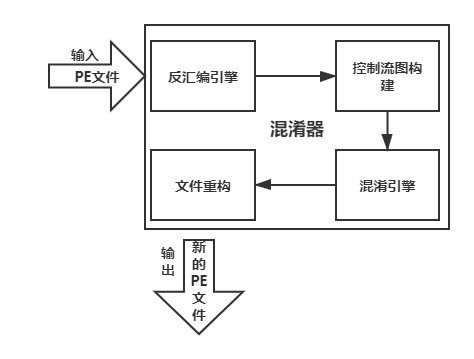
\includegraphics[width=8cm]{hunxiaoqi.png}
	\bicaption{混淆器总体结构}{The overall structure of the obfuscator}
	\label{hunxiaoqi}
\end{figure}

加壳器的输入为PE文件,输出为加壳后的PE文件。反汇编引擎模块对输入的PE文件进行反汇编,得到汇编代码;索引和控制流程把通过反汇编引擎得到的数据进行分析,处理程序的可交换函数、函数之间的调用情况、基本块的数量等信息;加密混淆引擎是整个处理流程的核心,根据索引和控制流程的信息,对程序进行函数混淆加密;文件重建是对混淆后的数据进行重构输出新的PE文件。

\subsection{二进制分析器设计与实现}
\label{san}

本节主要的内容是使用反汇编引擎对PE文件进行静态分析,为下节混淆器进行加密做准备。反汇编引擎使用OllyDbg的反汇编引擎,这个反汇编器是开源的,速度快,易于使用且稳定。由于本文提出的二进制混淆算法只处理MOV、SUB、ADD等不涉及堆栈和内存的混淆,属于非常基本混淆机制,没有复杂的内存处理,所有使用本反汇编引擎是最好的选择。

控制流程最主要的任务是建立基本块,如图\ref{jibenkuai}所示。

\begin{figure}[htbp]
	\centering
	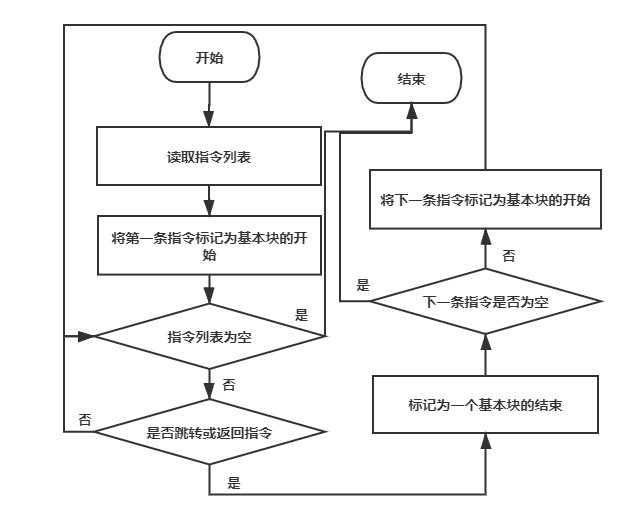
\includegraphics[width=11cm]{jibenkuai.png}
	\bicaption{基本块的识别过程}{Basic block recognition process}
	\label{jibenkuai}
\end{figure}

基本块的识别流程为:1.读取所有指令,标记起始指令;2.遍历指令列表,判断当前指令是否为返回指令或者跳转指令;3.如果不是跳转或返回指令则执行步骤2,进行下一条指令的遍历,否则将标记为基本块的结束;4.将下一条指令标记为另一个基本块的开始,跳转到2继续遍历其他所有指令。


\subsection{混淆器的设计与实现}


混淆器的编程实现难度偏高,故本文的实现中所参与交换的函数,不涉及处理内存、堆和栈中的数据,只处理交换函数之间的MOV、SUB、ADD等寄存器变换的指令。本文为了方便实现,将算法的某些细节进行简化,算法将不对函数进行详细分组,直接使用随机算法进行满足要求的函数,其中可能包含大量的MOV、SUB、ADD等基础指令并进行混淆。

\begin{figure}[htbp]
	\centering
	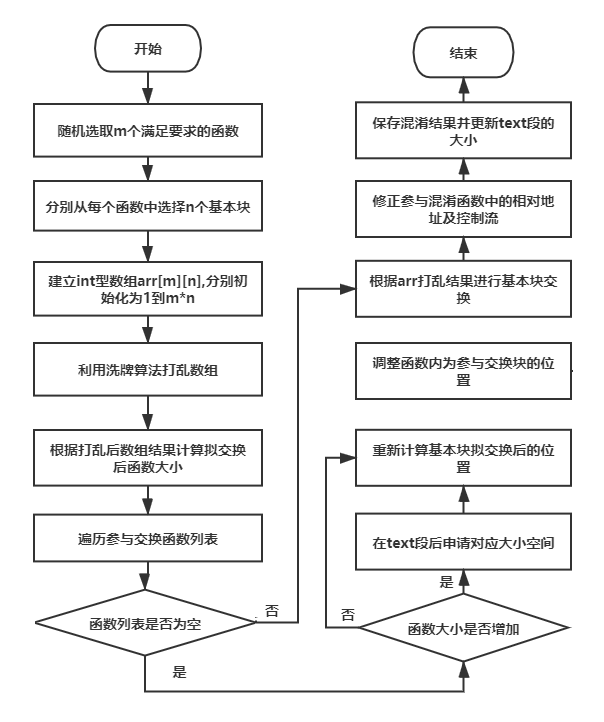
\includegraphics[width=13cm]{hunxiaoyinqing.png}
	\bicaption{混淆引擎工作原理}{How the obfuscation engine works}
	\label{hunxiaoyinqing}
\end{figure}

混淆器的工作流程如图\ref{hunxiaoyinqing},具体流程为:1.加密引擎首先根据二进制分析器提供的构建信息,从满足要求的函数中随机选取m个函数;2.将m个中选出的函数进行n个基本块之间的交换;3.建立一个long型数组arr[m*n],并进行1-m*n的初始化。4.使用Knuth\_Durstenfeld Shuffle算法对数组arr随机化;5.将函数产生的随机化数据进行如实交换;6.遍历参与混淆函数列表,如果为空,转到步骤11;7.判断函数的占用空间变化情况,如果没有变大,跳转到步骤9,否则在PE文件的最后加一个add节,并申请所需空间;9.计算出各个基本块交换后的新的位置,同时将交换索引放到PE文件中的add节中;10.保存处理过的指令,这里只处理了MOV指令;11.将arr数组的结果放到新的位置;12.修正函数的相对地址;13.保存混淆结果更新PE文件头,计算新添加节表的大小,并添加新add节表。

\subsection{二进制文件重建}

PE文件的重建工作是设计加壳器的重要一环,也是编程的瓶颈所在,PE文件重建,是根据加密结构重新建立一个PE文件,需要用到第二章提到过的大量内容。首先,肯定不能将混淆之后的汇编代码直接放到PE文件的各个段中,因为PE文件的各个段在经过加密之后占用空间大小会有所增加,PE文件头部的各个段大小需要修改。另外,各个段起始位置也都需要修改,否则可能会出现两个段重合。段中的跳转地址也需要相应的修复操作。将以上的信息进行修正之后,才能将修改后的汇编代码翻译成机器码写入到text段中重新生成一个PE文件。

%PE文件的重建模块流程如下图

%图
%所示。

PE文件重建步骤为:1.将混淆后的结果翻译成机器码,计算混合后的各个段的占用空间;2.更新PE文件头PE可选头表;3.检查混淆后代码段是否产生重叠,如果不重叠跳转到步骤5;4.将重叠的段向后移动;5.按照PE文件的布局依次将混淆后的结果依次写入到新的PE文件中,保存文件并退出。


%在面对软件保护技术的过程中由于许多软件开发人员仅专注于软件系统功能的实现,因此他们忽略了软件加密保护和反向破解。因此,在研究软件保护的初期,研究人员开发了一些相对有用的专业软件加密保护程序(简称Shell)。但是,随着破解技术的发展,甚至可以使用免费的OllyDbg删除使用强大的加密算法(例如Twofish,TEA,Blowfish以及CRC(循环冗余校验)和反调试技术的组合)的坚固外壳ASProtect。动态跟踪外壳后的反汇编代码。使用堆栈平衡原理在程序执行入口之前找到外壳,然后结合LoadPE工具的强大功能来导入表,导入地址表和重定位表。市面上大部分对软件的保护都基于上述的几种方式,本文将会在已有反调试基础上对已有算法进行优化改进。

%本课题实现的目标是对软件进行保护,防止未授权用户的非法注册,将分为两个大的设计模块,一方面对软件加入反跟踪调试技术,并对在目前流行的反跟踪调试基础上加入新的算法,以实现对非法用户的反编译混淆,另一方面对软件整体进行虚拟机加壳的方式进行保护,并在已有虚拟机Hanlder加密基础上进行动态加密解密,虚拟机加壳的方式是目前安全性能最高的方式,但是由于虚拟机保护方式需要在受保护的程序中加入虚拟机中字节码的解释器,因此在运行过程中会消耗大量的CPU时间,本文也会对加密后的程序的运行时间进行优化处理,尽可能提高程序的运行速度,并对已有虚拟机加壳进行对比。


%在试验阶段,将会使用不同的反编译器ODDBG、IDA、WinDbg)对加壳后的程序进行反汇编,对反调试性能和程序运行速度与市面流行保护引擎进行对比。由于Linux和Windows操作系统的PE(Portable Executable)文件结构完全不同,本课题的所有实验环境仅限于Windows操作系统下的PE文件,对Linux下的ELF文件并不能进行加壳保护。

%本文的主题是围绕反调试技术和虚拟机加壳技术,从用户角度和破解者角度分别给出不同情况的分析方案,并基于此建立了一个软件保护框架,为反调试技术提供良好的试验环境。整体的框架结构参考图~\ref{cha2:fig:framework}。其中自下而上,按照颜色划分,黄色:操作系统内核层,黄色:操作系统PE文件装载器,蓝色下层:逆向技术(动态分析、静态分析)和PE文件结构,蓝色上层:反跟踪技术和软件加壳(加密壳、虚拟机壳),绿色:用户接口API。除了操作系统层之外,每部分都将在后文依次介绍。


\label{cha2:sec:arch}

%软件工程中软件架构是整个系统的草图,在本节中,基于上面图~\ref{cha2:fig:framework}中所给出的结构中的操作系统PE文件装载器和Windows kernel层加以分析,并根据逆向分析技术和PE文件结构这两个层面分别阐述我们要实现的反调试算法架构设计。反调试是在应用程序代码内使用的一组技术,用于检测和阻止调试行为。这阻止了攻击者动态运行应用程序,试图了解它们的工作方式并更改应用程序内某些功能或检查的行为。反调试技术包括观察和检测内存,操作系统,进程信息以及将调试器连接到应用程序后与没有调试器时相比出现的延迟之间的细微差异。尽管有几种不同的反调试方法,但是使用的主要方法之一就是修改后的代码反调试。该技术将代码插入应用程序的多个位置,以主动搜索断点,调试器或调试技术。这些断点的检测可以通过分析整个应用程序操作过程中的代码修改,同时将其与预期值或规范进行比较来获得。检测到的差异会引发警报,从而可能导致更深入的调查。


\section{本章小结}

本章对常见的静态分析混淆技术进行了研究,对抗逆向中容易出现的问题进行了总结,分析了已有方法的优缺点,并提出一种建立函数索引进行函数间基本块交换的一种混淆方式,基于随机算法的二进制代码混淆算法,对算法的细节进行了详细的描述。最后根据提出的算法设计并实现了一个PE文件加壳器,本文实现了MOV、SUB、ADD等指令的交换方式在处理内存和堆栈区域上,在进行混淆之后,合理地还原程序的运行环境,就可以实现其他指令转化方法。









